\section{Building our own tracking system using routers and hotspots}
This section will include the advancements made in building and gathering of information about using routers and hotspots to make our own ILBS, a list of objectives can be seen below. The goal for this is enabling us to calculate the positioning of ourself and compare them to the position provided by Cisco.

\begin{itemize}
	\item Equipment Requirements
	\item Test Capabilities of the Router 
	\item Test Capabilities of the Access Points\ofx{is this all?}
\end{itemize}

An overview of the entire system can be seen in \cref{fig:OwnSetup}. One router and four access points are set up in our group rooms, such that it covers three group rooms.
\begin{figure}[H]
	\centering
	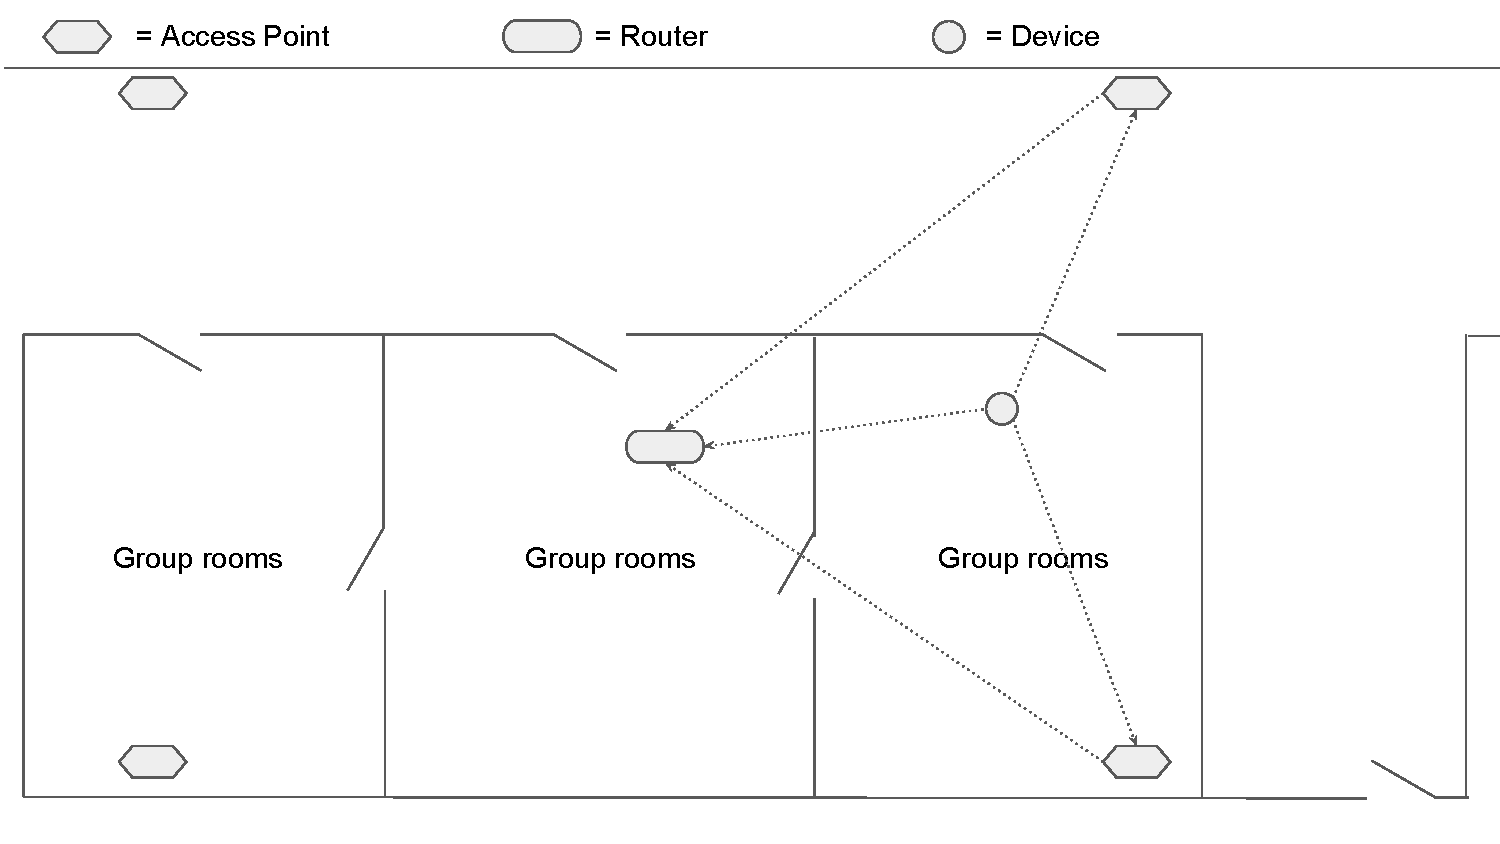
\includegraphics[scale=0.5]{graphics/Router-AccessPoint_Setup.pdf}
	\label{fig:OwnSetup}
	\caption{Illustration of how a positioning system can be set up using routers and access point that can track devices. \ofx{Any reason this is best?}}
\end{figure}

\subsection*{Equipment Requirements}
The initial requirements for the equipment, is a wireless antenna capable of supporting 2.4 GHz and optionally 5 GHz. It would be advantageously if we set up two different ILBS. We decided to buy two brands allowing us to analyse at least two ILBS and thus conclude which of the systems performed best, based on the criteria describe in section \ref{sec:monitoring}.

Based on the above requirement we found two brands, Ubiquiti and D-link which in comparison is considered the cheaper brand. We ordered one router, two expensive and five cheap access points of each brand.

\subsection*{Access point positioning}
Cisco\cite{access_point_placement} have guidelines for how to place the access points in order to get the best coverage with your system. They recommend that there are placed an access point in each corner of the building and some along the perimeter, if the building is large enough there should be placed some within the perimeter that can form a sub-perimeter in which there may be additional access points, this is illustrated in \cref{access_placement} on which the red circles is access points. Each access point should be place 50-70 feet away from each other in order to a high precision without a lot of unnecessary overlap\cite{access_point_range}.

\begin{figure}[H]
	\centering
	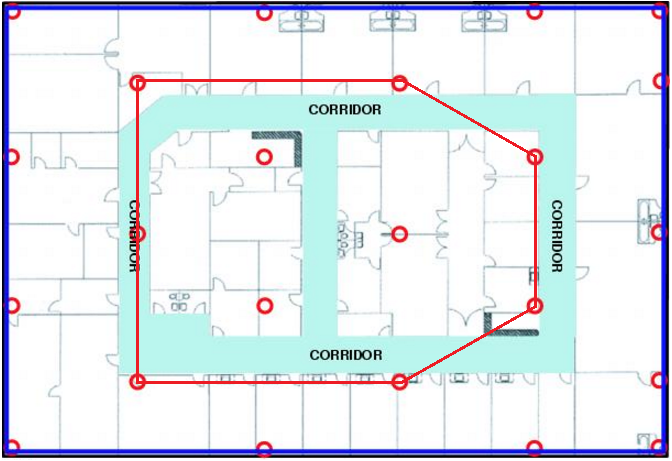
\includegraphics[scale=0.5]{graphics/access_placement.png}
	\label{fig:access_placement}
	\caption{Illustration of how access points should be placed.}
\end{figure}

\subsection*{Test Capabilities of the Equipment}
We tested the Ibiquiti equipment, with the original firmware. At first glance we are able to get transmission(TX) and receive(RX) signals of connected devices, unfortunately we do not receive the signals from devices not connected to the router. It was attempted to use the routers terminal which did not yield any results due to restricted access.

This caused us to research custom firmware for the router. By installing new firmware on the router we will be able to get root access to the router and thereby manipulate it at a lower level then the routers original firmware allows, this is necessary if we are to capture every receive signal the router gets.

We did find a custom firmware for Ibiquiti, however not for D-link. The searched sites were: openwrt.org{cite?}, polarcloud.com\ofx{cite?}, dd-wrt.com, gargolye-router.com\ofx{cite?}, librecmc.org\ofx{cite?} and wrtrouters.com\ofx{cite?}. These sites covers thousands of routers and the fact that we were not able to find a custom firmware for D-link might be because that the particular model we ordered\ofx{something is missing} because other routers from that brands were supported, nothing conclusion was found, to why it is not covered on any of the websites because\ofx{What?!}.

We ended up going with the openwrt because it supported our Ibiquiti router and allows us to gain root access and execute programs. With the new custom firmware installed we have around 8Mb of memory left this put some limitation to which language we can use, our first attempt is to use a version of python called mini-python that dose not exceed the memory limit.

A program is constructed allowing us to listen on different types of networks such as LAN and WAN, this is done using the socket library. We were however not able to import the library\ofx{which one?} required, to run the program on the router.